\chapter{Domain Model}

% Brief discussion of our model, ie MVC
As Capital Games is a very data-driven application, the database layer is
one of the most core concepts. Therefore, even though an end-user may
be interacting with only Leagues, only Orders, only Portfolios, or any
combination of the above, nearly every interaction with the system
involves at least one call to the database. Therefore, the domain model
is built around the data collections and abstractions involved in the site.
Above the database layer is a system layer which is responsible for both
interacting with the database layer as well as other core modules.

\section{Domain Model}
All models are attached in the next two pages.

\begin{figure}
\centering
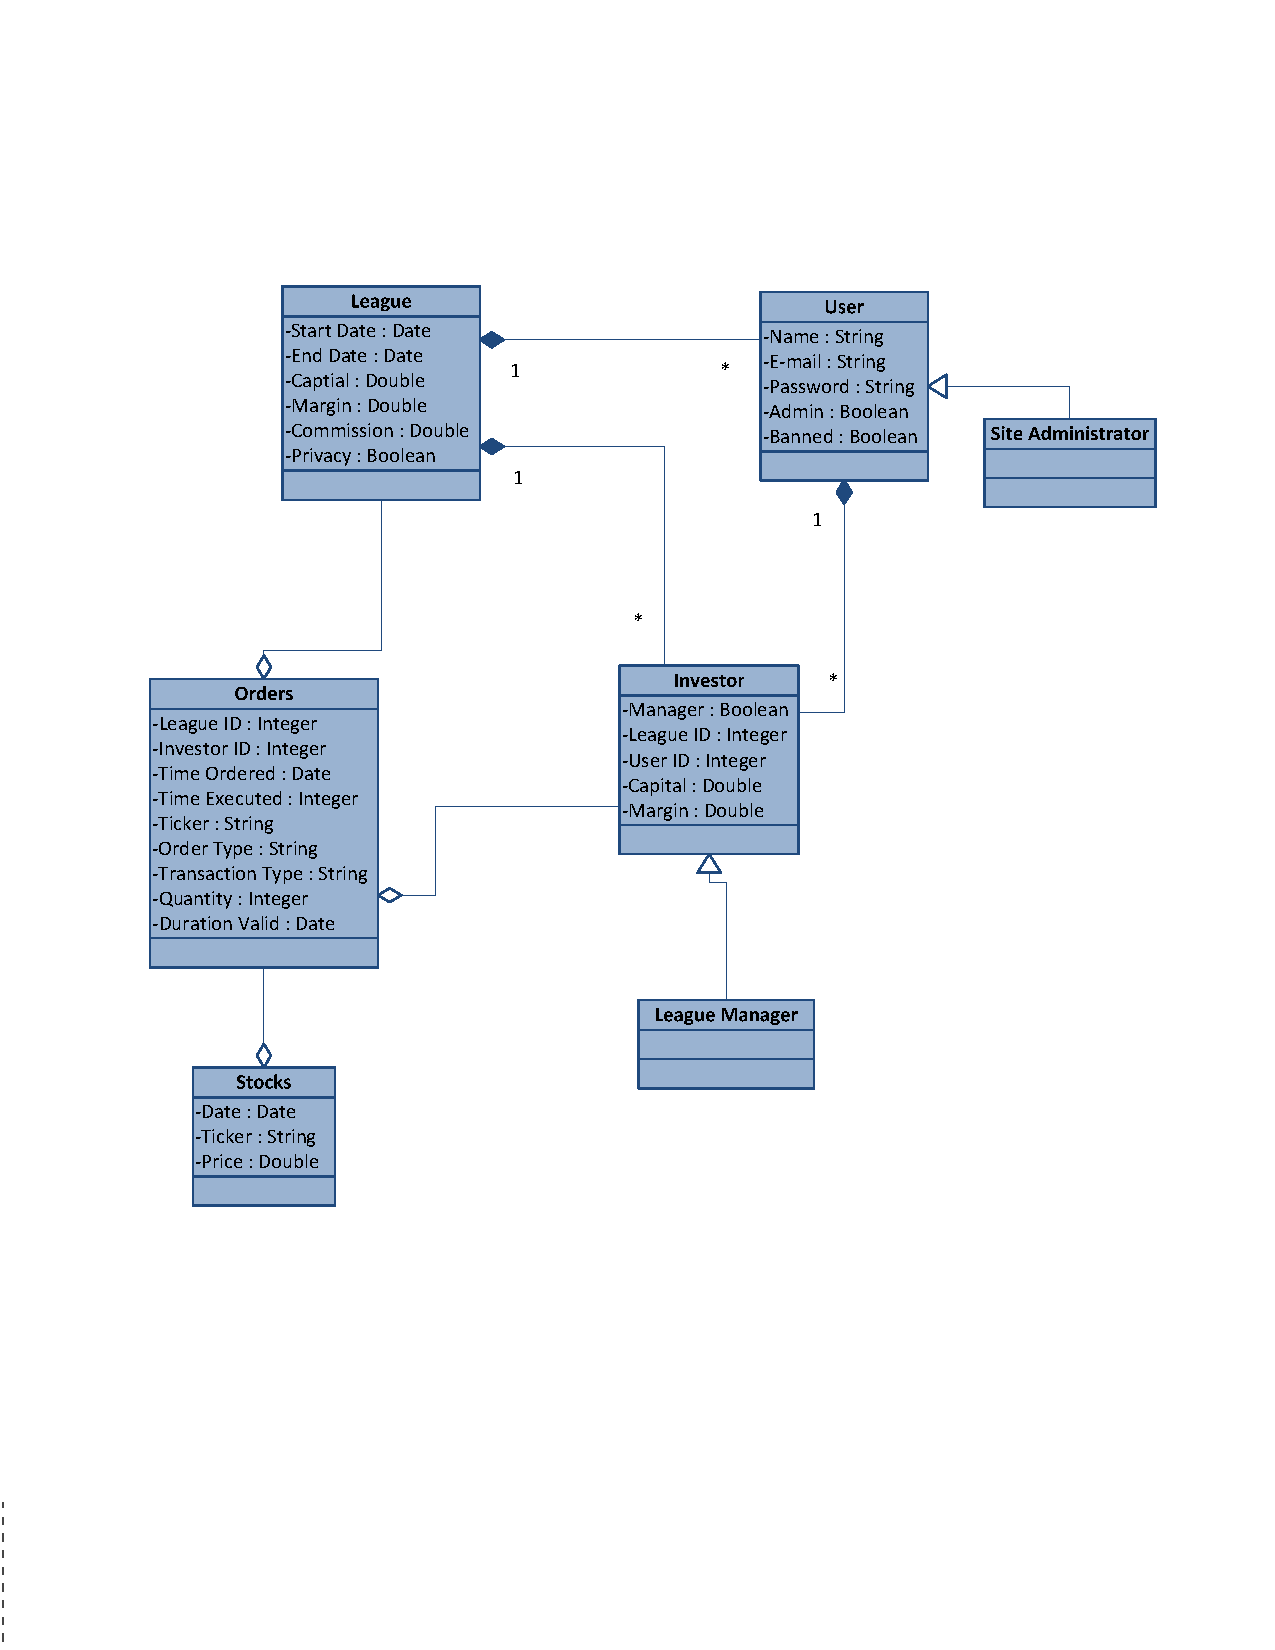
\includegraphics[width=5.5in]{./img/domainModel.pdf}
\caption{ }
\end{figure}

\section{Abstract Model}
\begin{figure}
\centering
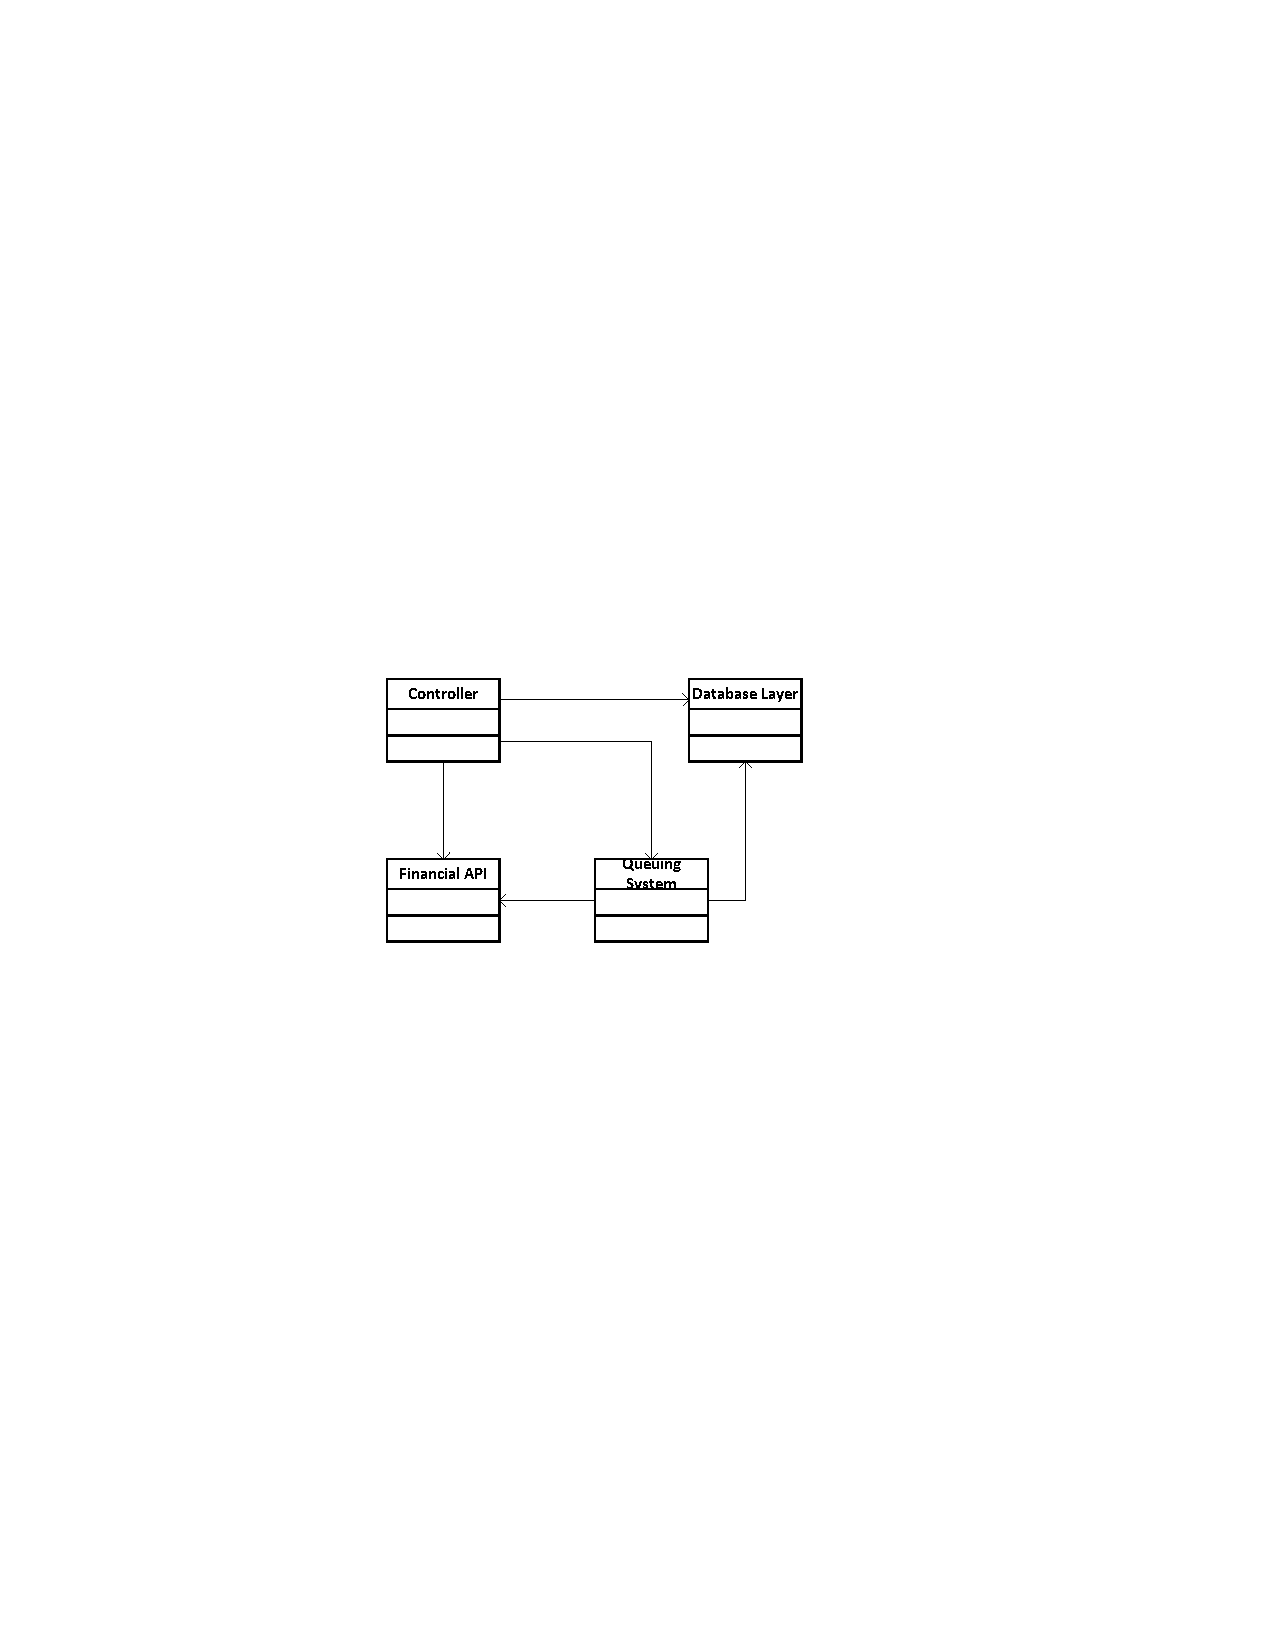
\includegraphics[width=5.5in]{./img/AbstractModel.pdf}
\caption{ }
\end{figure}

% Concept Definitions
\section{Concept Definitions}

From our Use Case analysis, we can immediately determine that several
actors have models in the application domain.

\begin{itemize}
\item \textbf{Users}: Every end-user of the application needs both a private and
public facing identity on the site.

\item \textbf{Site Administrators}: The site needs a few global administrators
who can delete posts and ban users which are innappropriate, as well
as perform several maintenance features.

\item \textbf{Leagues}: Every end-user is participating in one or more leagues.

\item \textbf{Investors}: Because an end-user can participate in multiple leagues,
and each instance of the user can have a separate amount of money, margin,
etc., it is necessary to maintain a separate identity for each of these 
instances -- \emph{investors}.

\item \textbf{League Manager}: Every League should have a superuser who is 
able to invite other players, perform moderation, and change settings.
\end{itemize}

Although not actors themselves, from UC-4 (page \pageref{UC-4}) and UC-5 
(page \pageref{UC-5}) it is apparent that end-users are implicitly 
requesting and manipulating data for their orders and portfolios. These,
too, become part of the application domain.

\begin{itemize}
\item \textbf{Orders}: When an \emph{Investor} places any type of order, it
needs to be tracked. 
\item \textbf{Stocks}: Whenever an Investor is tracking the performance of a
stock, those data need to be stored locally. Stocks is a unified 
data object to contain those data.
\end{itemize}

One of the actors at the back end of UC-3 (page \pageref{UC-3}) and UC-4
(\pageref{UC-4}) was the Financial API, responsible for accessing the 
market data stream. 

\begin{itemize}
\item \textbf{Financial API}: This module presents an interface for requesting market
data, both live and historical. 
\end{itemize}

Upon further analysis, it becomes apparent that the domain model is missing
functionality responsible for asynchronously executing jobs. This is another
core feature of the site, without which Stop and Limit Orders could not 
be placed.

\begin{itemize}
\item \textbf{Queueing System}: Many interactions need to be performed asynchronously,
such as the execution of Stop and Limit Orders and the delivery of e-mail 
updates. This module encapsulates the functionality of creating, maintaining,
and executing jobs which need to be performed asynchronously.
\end{itemize}

Finally, we need an abstraction for the part of the system which invokes and operates
upon the rest as a collective.

\begin{itemize}
\item \textbf{Controller}: The Controller is the model which receives requests from 
the end-user, interprets them, invokes other models and modules accordingly, and 
returns the response (when applicable).
\end{itemize}


% Association definitions between actors
\section{Association Definitions}

% brief discussion of how the parts relate to each other
Clearly, many of these models are interrelated. Below is a non-comprehensive
list of associations between various types of models.

\begin{itemize}
\item \textbf{Controller}: The Controller interacts with the collective database layer, 
as well as the other core modules.
	\begin{itemize}
	\item \textbf{Association}: Controller invokes the Database layer (and data contained therein)
	\item \textbf{Association}: Controller invokes the Financial API 
	\item \textbf{Association}: Controller invokes the Queueing System
	\end{itemize}
\item \textbf{Queuing System}: The Queueing System can almost be thought of as a 
miniature, self-regulating Controller. It can invoke the Financial API and the 
collective database layer.
	\begin{itemize}
	\item \textbf{Association}: Queueing System invokes the Financial API
	\item \textbf{Association}: Queueing System invokes the Database layer
	\end{itemize}
\item \textbf{Database Layer}: The Database Layer stores data into data objects and then
saves them to the underlying database. The Database Layer can perform limited checking
and updating logic when invoked, but is not self-regulating. It contains models of
several types of actors.
	\begin{itemize}
	\item \textbf{Users}: Represents end-users and their personal information
		\begin{itemize}
		\item \textbf{Inheritance}: Users is the parent class of Site Administrators
		\item \textbf{Aggregation}: Users have many Investors (User-Instances)
		\item \textbf{Composition}: Leagues have many Users
		\end{itemize}
	\item \textbf{Site Administrators}: A superclass of Users
		\begin{itemize}
		\item \textbf{Inheritance}: Site Administrators inherits from Users
		\end{itemize}
	\item \textbf{Leagues}: Represents simulation instances
		\begin{itemize}
		\item \textbf{Composition}: Leagues have many Users
		\item \textbf{Composition}: Leagues have many Investors (User-Instances)
		\item \textbf{Aggregation}: Leagues have many Orders
		\end{itemize}
	\item \textbf{Investors}: Represents User-Instances within Leagues
		\begin{itemize}
		\item \textbf{Composition}: A League has many Investors
		\item \textbf{Aggregation}: A User has many Investors
		\item \textbf{Aggregation}: An Investor has many Orders
		\end{itemize}
	\item \textbf{League Managers}: A superclass of Investors
		\begin{itemize}
		\item \textbf{Inheritance}: League Managers inherits from Investors
		\end{itemize}	
	\item \textbf{Orders}: Contains order data
		\begin{itemize}
		\item \textbf{Aggregation}: Leagues have many Orders
		\item \textbf{Aggregation}: Investors have many Orders
		\item \textbf{Association}: Orders are placed for Stocks
		\end{itemize}
	
		In addition, there are a few interesting types of orders, namely:
		\begin{itemize}
		\item \textbf{Market Order}: Orders executed immediately
		\item \textbf{Stop Order}: Orders executed after a certain price is exceeded
		\item \textbf{Limit Order}: Orders executed strictly beyond a certain price
		\end{itemize}
	\item \textbf{Stocks}: Contains data on stocks held by Investors
		\begin{itemize}
		\item \textbf{Association}: Orders are placed for stocks
		\end{itemize}
	\end{itemize}
\end{itemize}


% Attribute definitions
\section{Attribute Definitions}

It is clear from the domain model abstraction above that the Database Layer
models have many noteworthy attributes, and are heavily state-based. However,
the Financial API has no state, and is simply an aggregation of functionality.
Likewise with the Controller. Therefore, attributes are only elaborated on for
the Database Layer. 

\begin{itemize}
	\item \textbf{User}
		\begin{itemize}
		\item Name: String
		\item E-mail: String
		\item Password: String
		\item Admin: Bool
		\item Banned: Bool
		\end{itemize}
	\item \textbf{Investor}
		\begin{itemize}
		\item Manager: Bool
		\item League ID: Integer
		\item User ID: Integer
		\item Capital: Double
		\item Margin: Double
		\end{itemize}
	\item \textbf{League}
		\begin{itemize}
		\item Start Date: Date
		\item End Date: Date
		\item Capital: Double
		\item Margin: Double
		\item Commission: Double
		\item Privacy: Bool \footnote{To simplify joining private leagues, 
			we allow that whenever a User is ``invited'' to join one,
			an \emph{Investor} is created for them within that league, 
			granting immediate access.}
		\end{itemize}
	\item \textbf{Orders}
		\begin{itemize}
		\item League ID: Integer
		\item Investor ID: Integer
		\item Time Ordered: Date
		\item Time Executed: Date
		\item Ticker: String
		\item Order Type: String \footnote{Market, Stop, Limit}
		\item Transaction Type: String \footnote{Buy, Sell, Short, Cover}
		\item Quantity: Integer
		\item Duration Valid: Date
		\end{itemize}
	\item \textbf{Stocks}
		\begin{itemize}
		\item Date: Date
		\item Ticker: String
		\item Price: Double \footnote{Any other interesting metrics can likewise
			be stored here.}
		\end{itemize}
\end{itemize}

The Queueing System itself is an aggregation of functionality
present in the controller and operates on state data from the Database. However,
it is still under active development, and so a model for it has not yet been 
constructed. It could be one large, all-encompassing system, or (more likely)
will be split off into individual subsystems.

% put some BS here...

% Traceability Matrix
% This section can be implemented at your discretion,
% and to the extent you desire. We were already
% kind of waived out of having one, but maybe include
% the derivations of the domain model from the use cases
% or at least why an MVC style works. No need to go into
% too much detail about MVC though, because there's an
% architecture report due next week anyway...
% \section{Traceability Matrix}

% Put the Domain Model Graphic here: